%%%%%%%%%%%%%%%%%%%%%%%%%%%%%%%%%%%%%%%%%
%  My documentation report
%  Objective: Explain what I did and how, in order to help someone continue with the investigation
%
% Important note:
% Chapter heading images should have a 2:1 width:height ratio,
% e.g. 920px width and 460px height.
%
% The images can be found anywhere, usually on sky surveys websites or the
% Astronomy Picture of the day archive http://apod.nasa.gov/apod/archivepix.html
%
% The original template (the Legrand Orange Book Template) can be found here --> http://www.latextemplates.com/template/the-legrand-orange-book
%
% Original author of the Legrand Orange Book Template:
% Mathias Legrand (legrand.mathias@gmail.com) with modifications by:
% Vel (vel@latextemplates.com)
%
% Original License:
% CC BY-NC-SA 3.0 (http://creativecommons.org/licenses/by-nc-sa/3.0/)
%%%%%%%%%%%%%%%%%%%%%%%%%%%%%%%%%%%%%%%%%
 
%----------------------------------------------------------------------------------------
%	PACKAGES AND OTHER DOCUMENT CONFIGURATIONS
%----------------------------------------------------------------------------------------

\documentclass[11pt,fleqn]{book} % Default font size and left-justified equations

\usepackage[top=3cm,bottom=3cm,left=3.2cm,right=3.2cm,headsep=10pt,letterpaper]{geometry} % Page margins

\usepackage{xcolor} % Required for specifying colors by name
\definecolor{ocre}{RGB}{52,177,201} % Define the orange color used for highlighting throughout the book

% Font Settings
\usepackage{avant} % Use the Avantgarde font for headings
%\usepackage{times} % Use the Times font for headings
\usepackage{mathptmx} % Use the Adobe Times Roman as the default text font together with math symbols from the Sym­bol, Chancery and Com­puter Modern fonts

\usepackage{microtype} % Slightly tweak font spacing for aesthetics
\usepackage[utf8]{inputenc} % Required for including letters with accents
\usepackage[T1]{fontenc} % Use 8-bit encoding that has 256 glyphs

% Bibliography
\usepackage[style=alphabetic,sorting=nyt,sortcites=true,autopunct=true,babel=hyphen,hyperref=true,abbreviate=false,backref=true,backend=biber]{biblatex}
\addbibresource{bibliography.bib} % BibTeX bibliography file
\defbibheading{bibempty}{}

%%%%%%%%%%%%%%%%%%%%%%%%%%%%%%%%%%%%%%%%%
% This is based on the Legrand Orange Book
% Structural Definitions File
%
% The original template (the Legrand Orange Book Template) can be found here --> http://www.latextemplates.com/template/the-legrand-orange-book
%
% Original author of the Legrand Orange Book Template::
% Mathias Legrand (legrand.mathias@gmail.com) with modifications by:
% Vel (vel@latextemplates.com)
%
% Original License:
% CC BY-NC-SA 3.0 (http://creativecommons.org/licenses/by-nc-sa/3.0/)
%
%%%%%%%%%%%%%%%%%%%%%%%%%%%%%%%%%%%%%%%%%
%----------------------------------------------------------------------------------------
%	VARIOUS REQUIRED PACKAGES
%----------------------------------------------------------------------------------------

\usepackage{titlesec} % Allows customization of titles
\usepackage{graphicx} % Required for including pictures
\usepackage{lipsum} % Inserts dummy text
\usepackage{tikz} % Required for drawing custom shapes
\usepackage[english]{babel} % English language/hyphenation
\usepackage{enumitem} % Customize lists
\setlist{nolistsep} % Reduce spacing between bullet points and numbered lists
\usepackage{booktabs} % Required for nicer horizontal rules in tables
\usepackage{eso-pic} % Required for specifying an image background in the title page
\usepackage{bbm}
%----------------------------------------------------------------------------------------
%	MAIN TABLE OF CONTENTS
%----------------------------------------------------------------------------------------

\usepackage{titletoc} % Required for manipulating the table of contents

\contentsmargin{0cm} % Removes the default margin
% Chapter text styling
\titlecontents{chapter}[1cm] % Indentation
{\addvspace{15pt}\large\sffamily\bfseries} % Spacing and font options for chapters
{\color{ocre!60}\contentslabel[\Large\thecontentslabel]{1cm}\color{ocre}} % Chapter number
{}  
{\color{ocre!60}\normalsize\sffamily\bfseries\;\titlerule*[.5pc]{.}\;\thecontentspage} % Page number

% Section text styling
\titlecontents{section}[1cm] % Indentation
{\addvspace{5pt}\sffamily\bfseries} % Spacing and font options for sections
{\contentslabel[\thecontentslabel]{1cm}} % Section number
{}
{\sffamily\hfill\color{black}\thecontentspage} % Page number
[]

% Subsection text styling
\titlecontents{subsection}[2cm] % Indentation
{\addvspace{1pt}\sffamily\small} % Spacing and font options for subsections
{\contentslabel[\thecontentslabel]{1cm}} % Subsection number
{}
{\sffamily\;\titlerule*[.5pc]{.}\;\thecontentspage} % Page number
[] 

% subsubsection text styling
\titlecontents{subsubsection}[3.5cm] % Indentation
{\addvspace{1pt}\sffamily\small} % Spacing and font options for subsections
{\contentslabel[\thecontentslabel]{1.5cm}} % Subsection number
{}
{\sffamily\;\titlerule*[.5pc]{.}\;\thecontentspage} % Page number
[] 

%----------------------------------------------------------------------------------------
%	MINI TABLE OF CONTENTS IN CHAPTER HEADS
%----------------------------------------------------------------------------------------

% Section text styling
\titlecontents{lsection}[1cm] % Indentation
{\footnotesize\sffamily} % Font settings
{}
{}
{}

% Subsection text styling
\titlecontents{lsubsection}[2cm] % Indentation
{\addvspace{1pt}\sffamily\small} % Font settings
{}
{}
{}

% Subsubsection text styling
\titlecontents{lsubsubsection}[.5em] % Indentation
{\normalfont\footnotesize\sffamily} % Font settings
{}
{}
{}

%----------------------------------------------------------------------------------------
%	PAGE HEADERS
%----------------------------------------------------------------------------------------

\usepackage{fancyhdr} % Required for header and footer configuration

\pagestyle{fancy}
\renewcommand{\chaptermark}[1]{\markboth{\sffamily\normalsize\bfseries\chaptername\ \thechapter.\ #1}{}} % Chapter text font settings
\renewcommand{\sectionmark}[1]{\markright{\sffamily\normalsize\thesection\hspace{5pt}#1}{}} % Section text font settings
\fancyhf{} \fancyhead[LE,RO]{\sffamily\normalsize\thepage} % Font setting for the page number in the header
\fancyhead[LO]{\rightmark} % Print the nearest section name on the left side of odd pages
\fancyhead[RE]{\leftmark} % Print the current chapter name on the right side of even pages
\renewcommand{\headrulewidth}{0.5pt} % Width of the rule under the header
\addtolength{\headheight}{2.5pt} % Increase the spacing around the header slightly
\renewcommand{\footrulewidth}{0pt} % Removes the rule in the footer
\fancypagestyle{plain}{\fancyhead{}\renewcommand{\headrulewidth}{0pt}} % Style for when a plain pagestyle is specified

% Removes the header from odd empty pages at the end of chapters
\makeatletter
\renewcommand{\cleardoublepage}{
\clearpage\ifodd\c@page\else
\hbox{}
\vspace*{\fill}
\thispagestyle{empty}
\newpage
\fi}

%----------------------------------------------------------------------------------------
%	THEOREM STYLES
%----------------------------------------------------------------------------------------

\usepackage{amsmath,amsfonts,amssymb,amsthm} % For math equations, theorems, symbols, etc

\newcommand{\intoo}[2]{\mathopen{]}#1\,;#2\mathclose{[}}
\newcommand{\ud}{\mathop{\mathrm{{}d}}\mathopen{}}
\newcommand{\intff}[2]{\mathopen{[}#1\,;#2\mathclose{]}}
\newtheorem{notation}{Notation}[chapter]

%%%%%%%%%%%%%%%%%%%%%%%%%%%%%%%%%%%%%%%%%%%%%%%%%%%%%%%%%%%%%%%%%%%%%%%%%%%
%%%%%%%%%%%%%%%%%%%% dedicated to boxed/framed environments %%%%%%%%%%%%%%
%%%%%%%%%%%%%%%%%%%%%%%%%%%%%%%%%%%%%%%%%%%%%%%%%%%%%%%%%%%%%%%%%%%%%%%%%%%
\newtheoremstyle{ocrenumbox}% % Theorem style name
{0pt}% Space above
{0pt}% Space below
{\normalfont}% % Body font
{}% Indent amount
{\small\bf\sffamily\color{ocre}}% % Theorem head font
{\;}% Punctuation after theorem head
{0.25em}% Space after theorem head
{\small\sffamily\color{ocre}\thmname{#1}\nobreakspace\thmnumber{\@ifnotempty{#1}{}\@upn{#2}}% Theorem text (e.g. Theorem 2.1)
\thmnote{\nobreakspace\the\thm@notefont\sffamily\bfseries\color{black}---\nobreakspace#3.}} % Optional theorem note
\renewcommand{\qedsymbol}{$\blacksquare$}% Optional qed square

\newtheoremstyle{blacknumex}% Theorem style name
{5pt}% Space above
{5pt}% Space below
{\normalfont}% Body font
{} % Indent amount
{\small\bf\sffamily}% Theorem head font
{\;}% Punctuation after theorem head
{0.25em}% Space after theorem head
{\small\sffamily{\tiny\ensuremath{\blacksquare}}\nobreakspace\thmname{#1}\nobreakspace\thmnumber{\@ifnotempty{#1}{}\@upn{#2}}% Theorem text (e.g. Theorem 2.1)
\thmnote{\nobreakspace\the\thm@notefont\sffamily\bfseries---\nobreakspace#3.}}% Optional theorem note

\newtheoremstyle{blacknumbox} % Theorem style name
{0pt}% Space above
{0pt}% Space below
{\normalfont}% Body font
{}% Indent amount
{\small\bf\sffamily}% Theorem head font
{\;}% Punctuation after theorem head
{0.25em}% Space after theorem head
{\small\sffamily\thmname{#1}\nobreakspace\thmnumber{\@ifnotempty{#1}{}\@upn{#2}}% Theorem text (e.g. Theorem 2.1)
\thmnote{\nobreakspace\the\thm@notefont\sffamily\bfseries---\nobreakspace#3.}}% Optional theorem note

%%%%%%%%%%%%%%%%%%%%%%%%%%%%%%%%%%%%%%%%%%%%%%%%%%%%%%%%%%%%%%%%%%%%%%%%%%%
%%%%%%%%%%%%% dedicated to non-boxed/non-framed environments %%%%%%%%%%%%%
%%%%%%%%%%%%%%%%%%%%%%%%%%%%%%%%%%%%%%%%%%%%%%%%%%%%%%%%%%%%%%%%%%%%%%%%%%%
\newtheoremstyle{ocrenum}% % Theorem style name
{5pt}% Space above
{5pt}% Space below
{\normalfont}% % Body font
{}% Indent amount
{\small\bf\sffamily\color{ocre}}% % Theorem head font
{\;}% Punctuation after theorem head
{0.25em}% Space after theorem head
{\small\sffamily\color{ocre}\thmname{#1}\nobreakspace\thmnumber{\@ifnotempty{#1}{}\@upn{#2}}% Theorem text (e.g. Theorem 2.1)
\thmnote{\nobreakspace\the\thm@notefont\sffamily\bfseries\color{black}---\nobreakspace#3.}} % Optional theorem note
\renewcommand{\qedsymbol}{$\blacksquare$}% Optional qed square
\makeatother

% Defines the theorem text style for each type of theorem to one of the three styles above
\newcounter{dummy} 
\numberwithin{dummy}{section}
\theoremstyle{ocrenumbox}
\newtheorem{theoremeT}[dummy]{Theorem}
\newtheorem{problem}{Problem}[chapter]
\newtheorem{exerciseT}{Exercise}[chapter]
\theoremstyle{blacknumex}
\newtheorem{exampleT}{Example}[chapter]
\theoremstyle{blacknumbox}
\newtheorem{vocabulary}{Vocabulary}[chapter]
\newtheorem{definitionT}{Definition}[section]
\newtheorem{corollaryT}[dummy]{Corollary}
\newtheorem{claimT}[dummy]{Claim}
\newtheorem{lemmaT}[dummy]{Lemma}
\theoremstyle{ocrenum}
\newtheorem{proposition}[dummy]{Proposition}

%----------------------------------------------------------------------------------------
%	DEFINITION OF COLORED BOXES
%----------------------------------------------------------------------------------------

\RequirePackage[framemethod=default]{mdframed} % Required for creating the theorem, definition, exercise and corollary boxes

% Theorem box
\newmdenv[skipabove=7pt,
skipbelow=7pt,
backgroundcolor=black!5,
linecolor=ocre,
innerleftmargin=5pt,
innerrightmargin=5pt,
innertopmargin=5pt,
leftmargin=0cm,
rightmargin=0cm,
innerbottommargin=5pt]{tBox}

% Exercise box	  
\newmdenv[skipabove=7pt,
skipbelow=7pt,
rightline=false,
leftline=true,
topline=false,
bottomline=false,
backgroundcolor=ocre!10,
linecolor=ocre,
innerleftmargin=5pt,
innerrightmargin=5pt,
innertopmargin=5pt,
innerbottommargin=5pt,
leftmargin=0cm,
rightmargin=0cm,
linewidth=4pt]{eBox}	

% Definition box
\newmdenv[skipabove=7pt,
skipbelow=7pt,
rightline=false,
leftline=true,
topline=false,
bottomline=false,
backgroundcolor=gray!10,
linecolor=ocre,
innerleftmargin=5pt,
innerrightmargin=5pt,
innertopmargin=5pt,
innerbottommargin=5pt
leftmargin=0cm,
rightmargin=0cm,
linewidth=4pt,
]{dBox}	

% Corollary box
\newmdenv[skipabove=7pt,
skipbelow=7pt,
rightline=false,
leftline=true,
topline=false,
bottomline=false,
linecolor=gray,
backgroundcolor=gray!10,
innerleftmargin=5pt,
innerrightmargin=5pt,
innertopmargin=5pt,
innerbottommargin=10pt
leftmargin=0cm,
rightmargin=0cm,
linewidth=4pt]{cBox}

% Creates an environment for each type of theorem and assigns it a theorem text style from the "Theorem Styles" section above and a colored box from above
\newenvironment{theorem}{\begin{tBox}\begin{theoremeT}}{\end{theoremeT}\end{tBox}}
\newenvironment{exercise}{\begin{eBox}\begin{exerciseT}}{\hfill{\color{ocre}\tiny\ensuremath{\blacksquare}}\end{exerciseT}\end{eBox}}				  
\newenvironment{definition}{\begin{dBox}\begin{definitionT}}{\end{definitionT}\end{dBox}}	
\newenvironment{example}{\begin{exampleT}}{\hfill{\tiny\ensuremath{\blacksquare}}\end{exampleT}}		
\newenvironment{corollary}{\begin{cBox}\begin{corollaryT}}{\end{corollaryT}\end{cBox}}	
\renewenvironment{lemma}{\begin{cBox}\begin{lemmaT}}{\end{lemmaT}\end{cBox}}
\newenvironment{claim}{\begin{cBox}\begin{claimT}}{\end{claimT}\end{cBox}}	


%----------------------------------------------------------------------------------------
%	REMARK ENVIRONMENT
%----------------------------------------------------------------------------------------

\newenvironment{remark}{\par\vspace{10pt}\small % Vertical white space above the remark and smaller font size
\begin{list}{}{
\leftmargin=35pt % Indentation on the left
\rightmargin=25pt}\item\ignorespaces % Indentation on the right
\makebox[-2.5pt]{\begin{tikzpicture}[overlay]
\node[draw=ocre!60,line width=1pt,circle,fill=ocre!25,font=\sffamily\bfseries,inner sep=2pt,outer sep=0pt] at (-15pt,0pt){\textcolor{ocre}{R}};\end{tikzpicture}} % Orange R in a circle
\advance\baselineskip -1pt}{\end{list}\vskip5pt} % Tighter line spacing and white space after remark

%----------------------------------------------------------------------------------------
%	SECTION NUMBERING IN THE MARGIN
%----------------------------------------------------------------------------------------

\makeatletter
\renewcommand{\@seccntformat}[1]{\llap{\textcolor{ocre}{\csname the#1\endcsname}\hspace{1em}}}                    
\renewcommand{\section}{\@startsection{section}{1}{\z@}
{-4ex \@plus -1ex \@minus -.4ex}
{1ex \@plus.2ex }
{\normalfont\large\sffamily\bfseries}}
\renewcommand{\subsection}{\@startsection {subsection}{2}{\z@}
{-3ex \@plus -0.1ex \@minus -.4ex}
{0.5ex \@plus.2ex }
{\normalfont\sffamily\bfseries}}
\renewcommand{\subsubsection}{\@startsection {subsubsection}{3}{\z@}
{-2ex \@plus -0.1ex \@minus -.2ex}
{.2ex \@plus.2ex }
{\normalfont\small\sffamily\bfseries}}                        
\renewcommand\paragraph{\@startsection{paragraph}{4}{\z@}
{-2ex \@plus-.2ex \@minus .2ex}
{.1ex}
{\normalfont\small\sffamily\bfseries}}

%----------------------------------------------------------------------------------------
%	HYPERLINKS IN THE DOCUMENTS
%----------------------------------------------------------------------------------------

% For an unclear reason, the package should be loaded now and not later
\usepackage{hyperref}
\hypersetup{hidelinks,backref=true,pagebackref=true,hyperindex=true,colorlinks=true,linkcolor=ocre,breaklinks=true,urlcolor= ocre,bookmarks=true,bookmarksopen=false,pdftitle={Introduction to Machine Learning (67577) - Course Book},pdfauthor={Author}}

%----------------------------------------------------------------------------------------
%	CHAPTER HEADINGS
%----------------------------------------------------------------------------------------

% The set-up below should be (sadly) manually adapted to the overall margin page septup controlled by the geometry package loaded in the main.tex document. It is possible to implement below the dimensions used in the goemetry package (top,bottom,left,right)... TO BE DONE

\newcommand{\thechapterimage}{}
\newcommand{\chapterimage}[1]{\renewcommand{\thechapterimage}{#1}}

% Numbered chapters with mini tableofcontents
\def\thechapter{\arabic{chapter}}
\def\@makechapterhead#1{
\thispagestyle{empty}
{\centering \normalfont\sffamily
\ifnum \c@secnumdepth >\m@ne
	\if@mainmatter
		\startcontents
		\begin{tikzpicture}[remember picture,overlay]
		\node at (current page.north west)
		{\begin{tikzpicture}[remember picture,overlay]
			\node[anchor=north west,inner sep=0pt] at (0,0) {\includegraphics[width=\paperwidth]{\thechapterimage}};
			%%%%%%%%%%%%%%%%%%%%%%%%%%%%%%%%%%%%%%%%%%%%%%%%%%%%%%%%%%%%%%%%%%%%%%%%%%%%%%%%%%%%%
			% Commenting the 3 lines below removes the small contents box in the chapter heading
			%\fill[color=ocre!10!white,opacity=.6] (1cm,0) rectangle (8cm,-7cm);
			%\node[anchor=north west] at (1.1cm,.35cm) {\parbox[t][8cm][t]{6.5cm}{\huge\bfseries\flushleft \printcontents{l}{1}{\setcounter{tocdepth}{2}}}};
			\draw[anchor=west] (5cm,-9cm) node [rounded corners=20pt,fill=ocre!10!white,text opacity=1,draw=ocre,draw opacity=1,line width=1.5pt,fill opacity=.6,inner sep=12pt]{\huge\sffamily\bfseries\textcolor{black}{\thechapter. #1\strut\makebox[22cm]{}}};
			%%%%%%%%%%%%%%%%%%%%%%%%%%%%%%%%%%%%%%%%%%%%%%%%%%%%%%%%%%%%%%%%%%%%%%%%%%%%%%%%%%%%%
			\end{tikzpicture}};
		\end{tikzpicture}}
\par\vspace*{270\p@}
\fi
\fi}

% Unnumbered chapters without mini tableofcontents (could be added though) 
\def\@makeschapterhead#1{
\thispagestyle{empty}
{\centering \normalfont\sffamily
\ifnum \c@secnumdepth >\m@ne
\if@mainmatter
\begin{tikzpicture}[remember picture,overlay]
\node at (current page.north west)
{\begin{tikzpicture}[remember picture,overlay]
\node[anchor=north west,inner sep=0pt] at (0,0) {\includegraphics[width=\paperwidth]{\thechapterimage}};
\draw[anchor=west] (5cm,-9cm) node [rounded corners=20pt,fill=ocre!10!white,fill opacity=.6,inner sep=12pt,text opacity=1,draw=ocre,draw opacity=1,line width=1.5pt]{\huge\sffamily\bfseries\textcolor{black}{#1\strut\makebox[22cm]{}}};
\end{tikzpicture}};
\end{tikzpicture}}
\par\vspace*{230\p@}
\fi
\fi
}
\makeatother % Insert the commands.tex file which contains the majority of the structure behind the template

\newcommand{\R}{\mathbb{R}}
\newcommand{\E}{\mathbb{E}}
\newcommand{\P}{\mathbb{P}}

\newcommand{\X}{\mathcal{X}}
\newcommand{\Y}{\mathcal{Y}}
\newcommand{\H}{\mathcal{H}}
\newcommand{\N}{\mathcal{N}}

\newcommand{\e}{$\varepsilon$} % Insert mathematics and notations 

\begin{document}
\title{Introduction to Machine Learning (67577) - Course Book - Edition 1}

%----------------------------------------------------------------------------------------
%	TITLE PAGE
%----------------------------------------------------------------------------------------

\begingroup
\thispagestyle{empty}
\AddToShipoutPicture*{\put(0,0){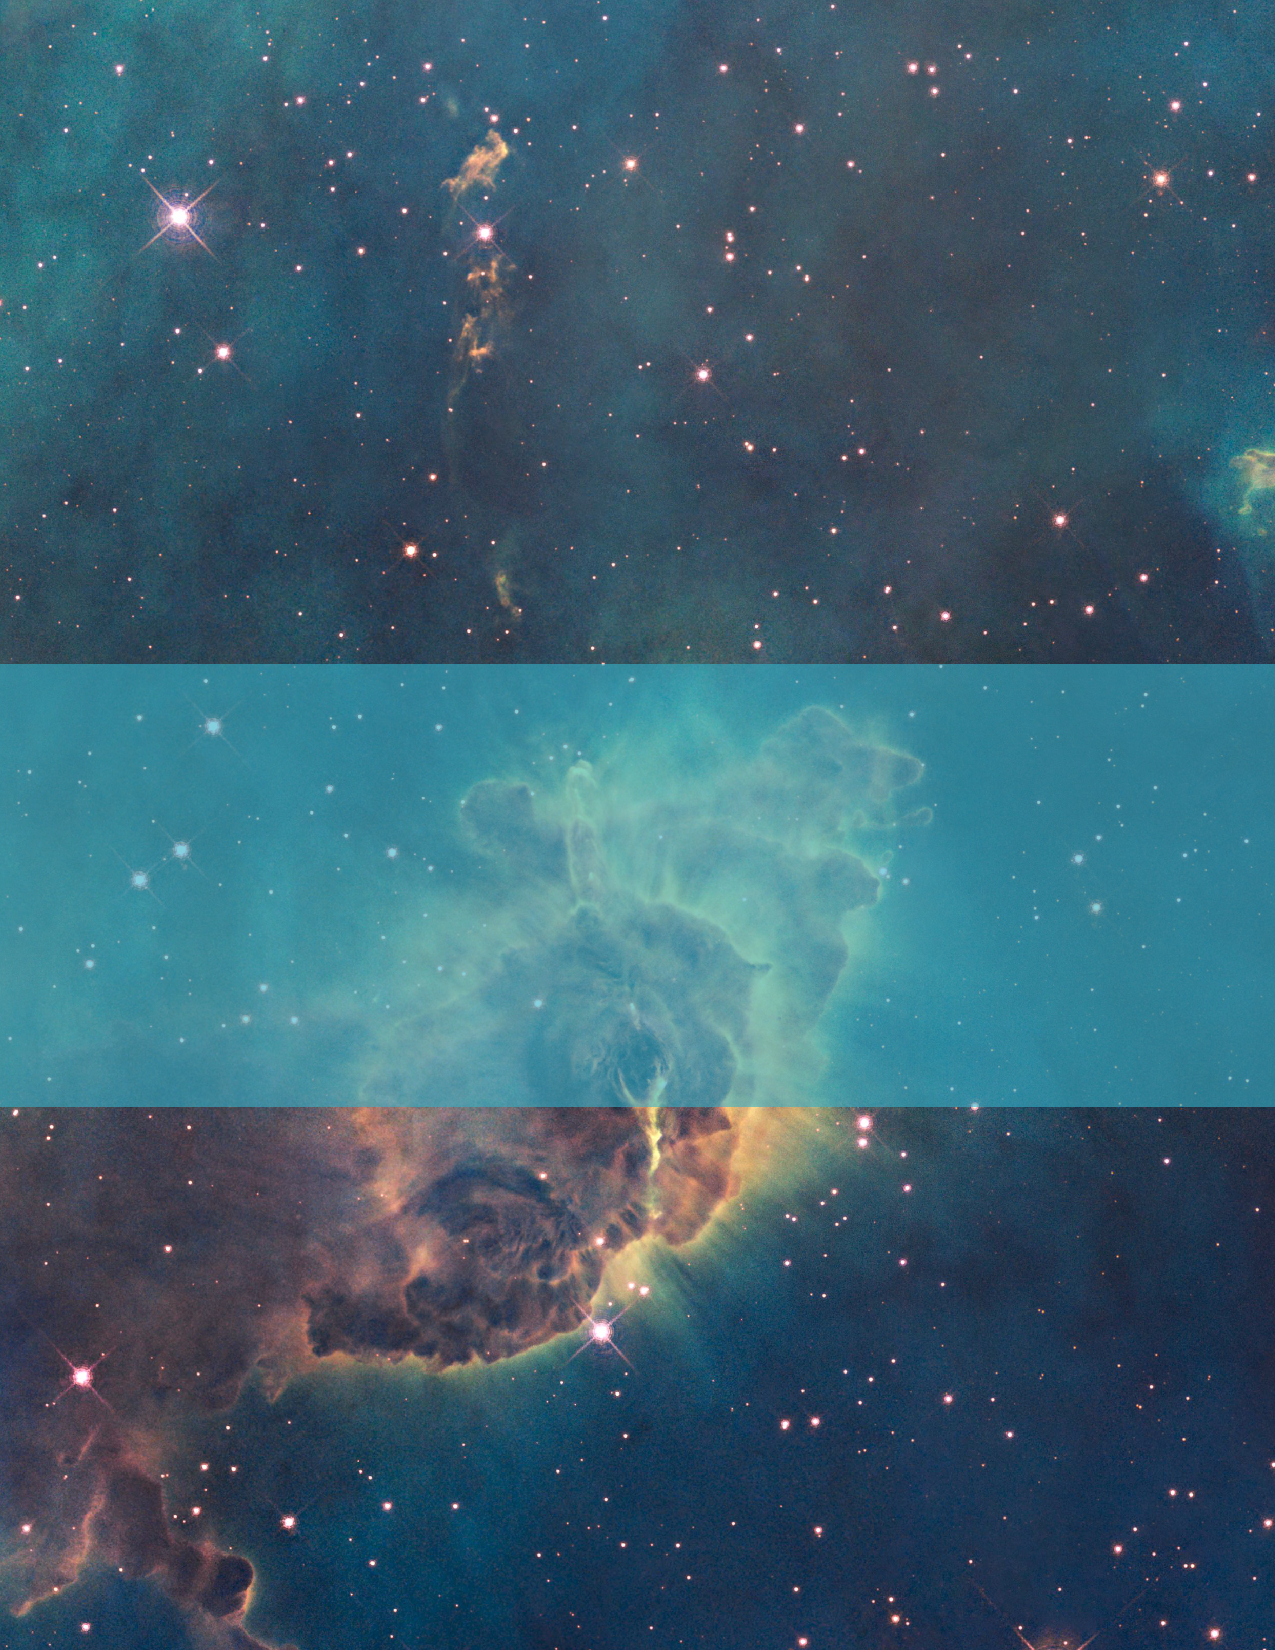
\includegraphics[scale=1.25]{esahubble}}} % Image background
\centering
\vspace*{5cm}
\par\normalfont\fontsize{35}{35}\sffamily\selectfont
\textbf{Introduction to Machine Learning}\\
{\LARGE 67577\\Course Book}\par % Book title
\vspace*{1cm}
%{\Huge Andrea Hidalgo}\par % Author name
\endgroup

%----------------------------------------------------------------------------------------
%	COPYRIGHT PAGE
%----------------------------------------------------------------------------------------

\newpage
~\vfill
\thispagestyle{empty}
%\noindent Copyright \copyright\ 2014 Andrea Hidalgo\\ % Copyright notice
\noindent \textsc{Introduction to Machine Learning, The Hebrew University, Jerusalem}\\

\noindent \textsc{Address to code examples and labs repository}\\ % URL

\noindent Written by and by.\\ % License information

\noindent \textit{First release, October 2020} % Printing/edition date

%----------------------------------------------------------------------------------------
%	TABLE OF CONTENTS
%----------------------------------------------------------------------------------------

\chapterimage{head1.png} % Table of contents heading image
\pagestyle{empty} % No headers
\tableofcontents % Print the table of contents itself
\cleardoublepage % Forces the first chapter to start on an odd page so it's on the right
\pagestyle{fancy} % Print headers again

\chapter{Mathematical Basis}
    \section{Linear Algebra}
        \subsection{Hyperplanes}
        \subsection{Projecting Matrices}
        \subsection{Matrix Decomposition}
            \subsubsection{Eigenvalues Decomposition}
            \subsubsection{Singular Values Decomposition}
    \section{Calculus}
        \subsection{High Order Derivatives}
        \subsection{Convexity}
    \section{Probabilities Theory}
        \subsection{Distributions and Random Variables}
        \subsection{Multi-variate Distributions}
        \subsection{Joint- and Marginal Distributions}
        \subsection{PDF and CDF of Distributions}
        \subsection{Measurements Of Concentration}

\chapter{Introduction \& Linear Regression}
    \section{Introduction to Statistical Learning}
        \subsection{Estimation Theory}
            \subsubsection{Estimators}
            \subsection{Risk \& Loss Functions}
        \subsection{Learning Principals}
            \subsubsection{Empirical Risk Minimization}
            \subsubsection{Maximum Likelihood}
        \subsection{Lab: Python Data Analysis - First Steps}
        \subsection{Lab: Data Simulation and Sampling}
        
    \section{Linear Regression}
        \subsection{Ordinary Least Squares}
        \subsection{Weighted Least Squares}
        \subsection{Geometric Interpretation}
        \subsection{Categorical Variables}
        \subsection{Lab: Linear Regression}
        
    \section{Beyond Linearity}
        \subsection{Polynomial Fitting}
        \subsection{Poisson Regression}
        \subsection{Lab: Polynomial Fitting}
    
\chapter{Classification}
    \section{Classification Overview}
        \subsection{Loss Function}
        \subsection{Type-I and Type-II Errors}
        \subsection{Statistical Measures of Performance}
        
    \section{Logistic Regression}
        \subsection{A Probabilistic Model For Noisy Labels}
            \subsubsection{The Hypothesis Class}
            \subsubsection{Learning Via Maximum Likelihood}
        \subsection{Computational Implementation}
        \subsection{Interpretability}
        \subsection{ROC Curve}
        \subsection{Lab: Logistic Regression}
    
    \section{Half-Space Classifier}
        \subsection{Learning Linearly Separable Data Via ERM}
        \subsection{Computational Implementation}
        \subsection{The Perceptron Algorithm}
        
    \section{Support Vector Machines}
        \subsection{Maximum Margin Learning Principal}
        \subsection{Hard-SVM}
        \subsection{Soft-SVM}
            \subsubsection{The Kernel Trick}
        
    \section{Nearest Neighbors}
        \subsection{Graph-Based Approach For Learning}
        \subsection{Classification \& Regression Using $k$-NN}
        \subsection{Computational Implementation}
        \subsection{Selecting Value of $k$ Hyper-Parameter}
        \subsection{Variants of Nearest Neighbors}
        
    \section{Decision Trees}
        \subsection{Axis-Parallel Partitioning of $\R^d$}
        \subsection{Classification \& Regression Trees}
        \subsection{Growing a Classification Tree}
        \subsection{NP-Hardness and CART Heuristic}
        \subsection{Pruning a Decision Tree}
    
    \section{Bayes Classifiers}
        \subsection{Bayes Optimal Classifier}
        \subsection{Naive Bayes}
        \subsection{Linear Discriminant Analysis}
        \subsection{Quadratic Discriminant Analysis}
        \subsection{Lab: Maximum Likelihood Estimation}
        
\chapter{PAC Theory of Statistical Learning}
    \section{Theoretical Framework For Learning}
        \subsection{Data-Generation Model}
        \subsection{The Realizability Assumption}
        \subsection{Learning As A Game - First Attempt}
        \subsection{Probably- and Approximately Correct Learners}
    \section{No Free Lunch and Hypothesis Classes}
        \subsection{No Free Lunch!}
        \subsection{Restricting for Hypothesis Classes}
        \subsection{Learning As A Game - Final Attempt}
        \subsection{Example: Threshold Functions}
    
    \section{PAC Learnability of Finite Hypothesis Classes}
    
    \section{VC-Dimension}
        \subsection{Formal Definition}
        \subsection{VC-Dimension of Finite Hypothesis Classes}
        \subsection{Example: Axis Aligned Rectangles}
        \subsection{Example: Half-Spaces}
        
    \section{Agnostic PAC: Extending Framework}
        \subsection{Data-Generation Model Over \X\times\Y}
        \subsection{Relaxing Realizability Assumption}
        \subsection{Introducing General Loss Functions}
        \subsection{Agnostic PAC Learnability}
    
    \section{Uniform Convergence Property}
        \subsection{\e-Representative Datasets}
        \subsection{Achieving Uniformity In \H and \D}
            \subsubsection{The Case Of Finite \H}
            \subsubsection{The General Case - Infinite \H}
    
    \section{The Fundamental Theorem of Statistical Learning}
    
\chapter{Ensemble Methods}
    \section{Bias-Variance Trade-off}
        \subsection{Generalization Error Decomposition}
        \subsection{Lab: Bias-Variance Via Decision Trees}
        \subsection{Lab: Bias-Variance Via Polynomial Fitting}
        
    \section{Ensemble/Committee Methods}
        \subsection{Weak-Learnability}
        \subsection{Uncorrelated Predictors}
        \subsection{Correlated Predictors}
        \subsection{Committee Methods In Machine Learning}
    
    \section{Boosting Weak-Learners}
        \subsection{AdaBoost Algorithm}
        \subsection{Gradient Boosting Algorithm}
        \subsection{Lab: Boosting - Image Classification}
        
    \section{Bagging}
        \subsection{Bootstrapping}
            \subsubsection{} % wider use
        \subsection{Bagging Reduces Variance}
        \subsection{Random Forests Bagging and De-correlating Decision Trees}
        
\chapter{Regularization, Model Selection and Model Evaluation}
    \section{Regularization}
        \subsection{Best Subset Selection}
        \subsection{$L_q$ Nrom Regularizes}
            \subsection{Ridge Regularization}
            \subsection{Convexity vs. Sparsity}
            \subsection{Lasso Regularization}
        \subsection{Lab: Regularized Logistic Regression}
    
    \section{Model Selection and -Evaluation}
        \subsection{Cross Validation}
        \subsection{Bootstrap}
        \subsection{Common Model Selection Mistakes}
            \subsubsection{Over-estimating Generalization Error}
            \subsubsection{Under-estimating Generalization Error}
    \subsection{Lab: Selecting Regularized Model}
        
\chapter{Unsupervised Learning}
    \section{Dimensionality Reduction}
        \subsection{Preserved Data Properties}
        \subsection{Principal Component Analysis}
            \subsubsection{Closest Subspace Interpretation}
            \subsubsection{Generalized Linear Regression Interpretation}
            \subsubsection{Maximum Retained Variance Interpretation}
            \subsubsection{Projection- vs. Coordinates of Data-Points}
            \subsubsection{Variants of PCA}
        \subsubsection{Euclidean Embedding}
        \subsection{Lab: PCA}
        
    \section{Clustering}
        \subsection{K-Means}
            \subsubsection{}
            \subsubsection{K-Means++}
        \subsection{Mixture of Gaussians}
            \subsubsection{Expectation Minimization Learning Principal}
            \subsubsection{Estimating Model Parameters}
        \subsection{Spectral Clustering}
        \subsection{Lab: K-Means++}
        \subsection{Lab: Parameters Estimation In MoG}
    
\chapter{Convex Optimization and Gradient Descent}
    \subsection{Gradient Descent Learning Principal}
    \subsection{Utilizing Sub-gradients For GD}
    \subsection{Stochastic Gradient Descent}
    \subsection{Variants Of Gradient Descent}
        \subsection{Initialization Conditions}
        \subsection{Tuning Learning Rates}

\chapter{Online- and Reinforcement Learning}
\chapter{Deep Learning}

\newpage
\end{document}